\subsection{Motion Retargeting for Avatar Adaptation}
\label{sec:retargeter}

Retargeting adapts processed motion data to a specific avatar format.
This process enables custom avatar expression or subsequent steps in the processing pipeline to apply format-specific adjustments.
The primary goal is to transfer motion to the avatar format, minimizing the discrepancy between the original motion and the avatar's representation while ensuring that the resulting animation is natural.
Although conventional methods often tightly couple the retargeting logic with a specific SDK or do not provide comprehensive retargeting methods, our approach decouples these components.
This separation allows for multiple expressions to various avatar rigs within the same graph computation, irrespective of the underlying XR SDK (see {\bf Figure~\ref{fig:retarget}}).

\subsubsection{Retarget Manager}
The Retarget Manager coordinates the registered Retargeter components.
Actual retargeting logic, which converts computed motion to the avatar format, is executed by individual Retargeter components managed by the Retarget Manager.
The retargeting logic is detailed in the following paragraphs.
The manager integrates its outputs, applying the final motion to the custom avatar skeleton and, if necessary, using forward kinematics (FK).

\subsubsection{Body Skeleton Retargeting}
As Motion Nodes, each Retargeter is responsible for matching published motion data to a specific part of the target avatar rig.
Individual Retargeters handle different body parts and tracking modalities according to their subscribed publishers.
For hardware-based trackers, user-controllable tracker-rotation correction is provided through a Retargeter to handle device-specific orientation adjustments.
For software-based tracking and estimation methods enhanced by ML, Retargeters rely on reference avatar frames to establish correspondence.
The principle of this retargeting approach is to establish anatomical foundations that enable the mapping of relative transformations.
Let $\mathbf{T}_{j,\mathrm{src}}^0$ and $\mathbf{T}_{j,\mathrm{src}}(t)$ denote the homogeneous transforms of source joint $j$ at the canonical T-pose and at time $t$, and let $\mathbf{T}_{j,\mathrm{tgt}}^0$ denote the target avatar's T-pose transform.
All transforms are world-frame homogeneous transforms, using column vectors and left-multiplication (x' = T x)
The Retargeter applies the relative motion
\begin{equation}
    \mathbf{T}_{j,\mathrm{tgt}}(t) = \mathbf{T}_{j,\mathrm{src}}(t)\,\mathbf{A}_j\,\mathbf{T}_{j,\mathrm{tgt}}^0,
\end{equation}
where $\mathbf{A}_j = \big(\mathbf{T}_{j,\mathrm{src}}^0\big)^{-1}$ denotes the conceptual alignment operator from the source canonical pose.
In practice, the runtime applies equivalent alignment through direct transform composition rather than storing a separate $\mathbf{A}_j$ variable.

\subsubsection{XR Hand Retargeter: Anatomical Frames}

\begin{figure}[!t]
    \centering
    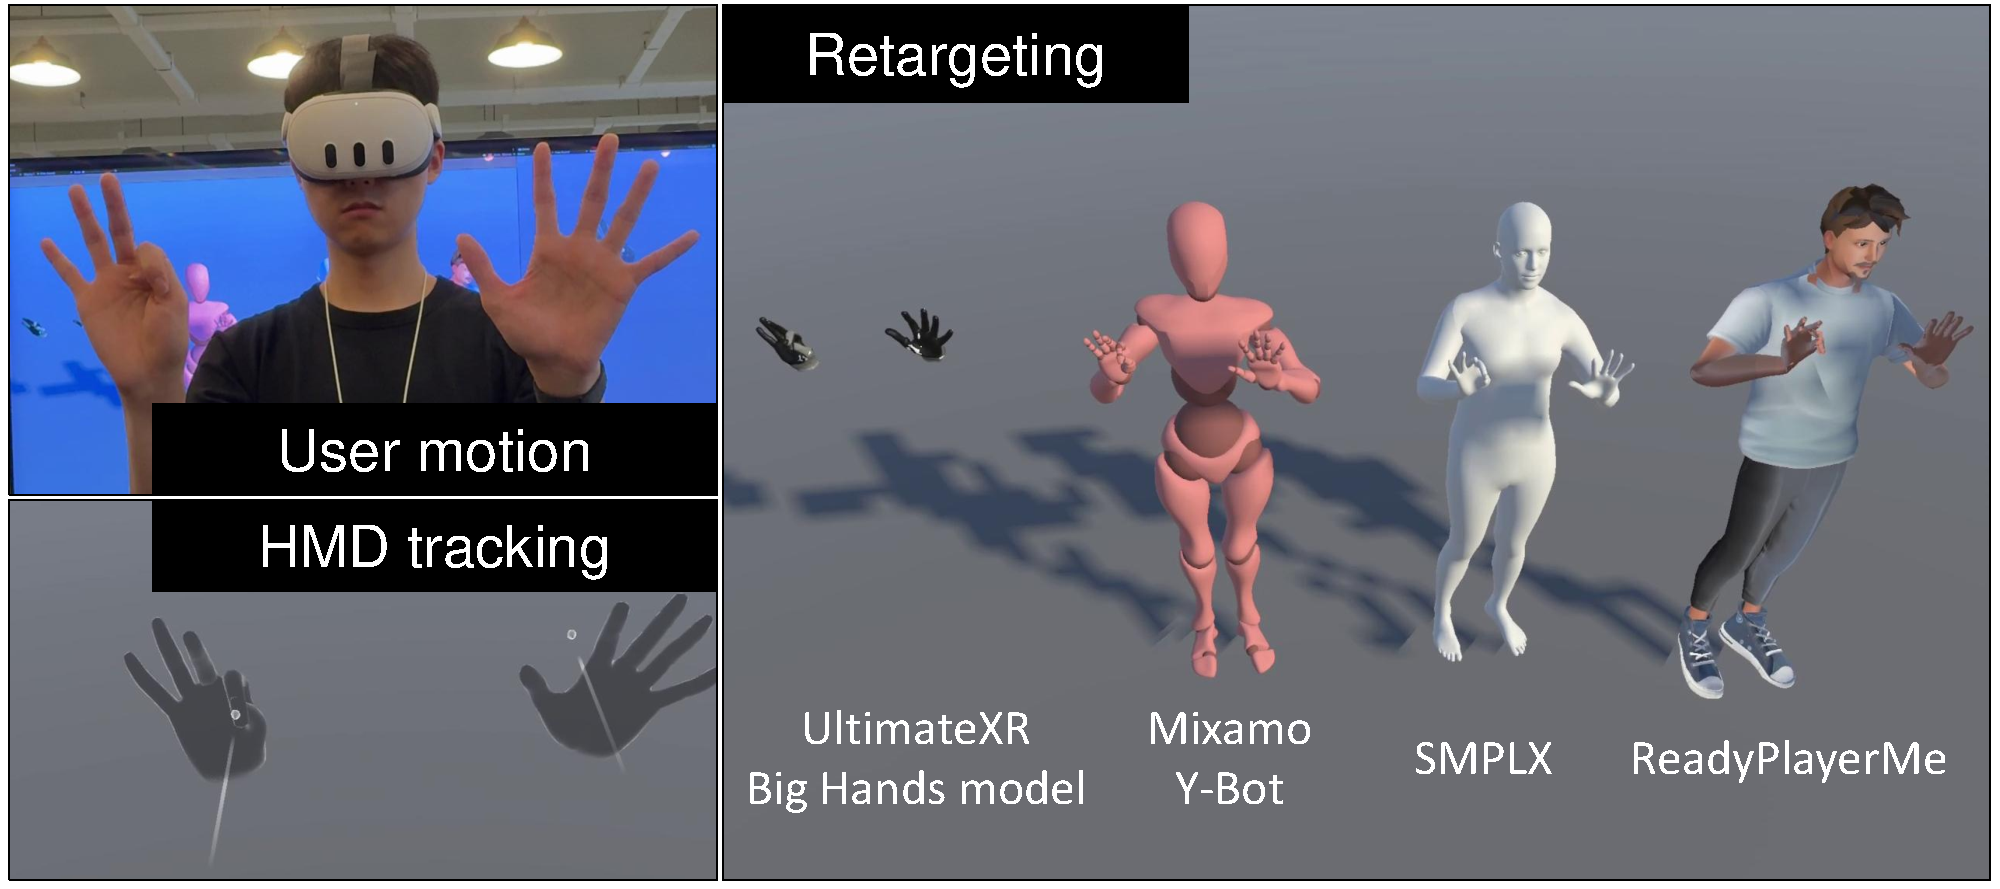
\includegraphics[width=\columnwidth]{figures/fig3-retarget.pdf}
    \caption{Retargeting results from 3-DoF HMD-based tracking to heterogeneous avatar representations using MotionDAG.}
    \label{fig:retarget}
\end{figure}


\begin{figure*}[ht]
  \centering
  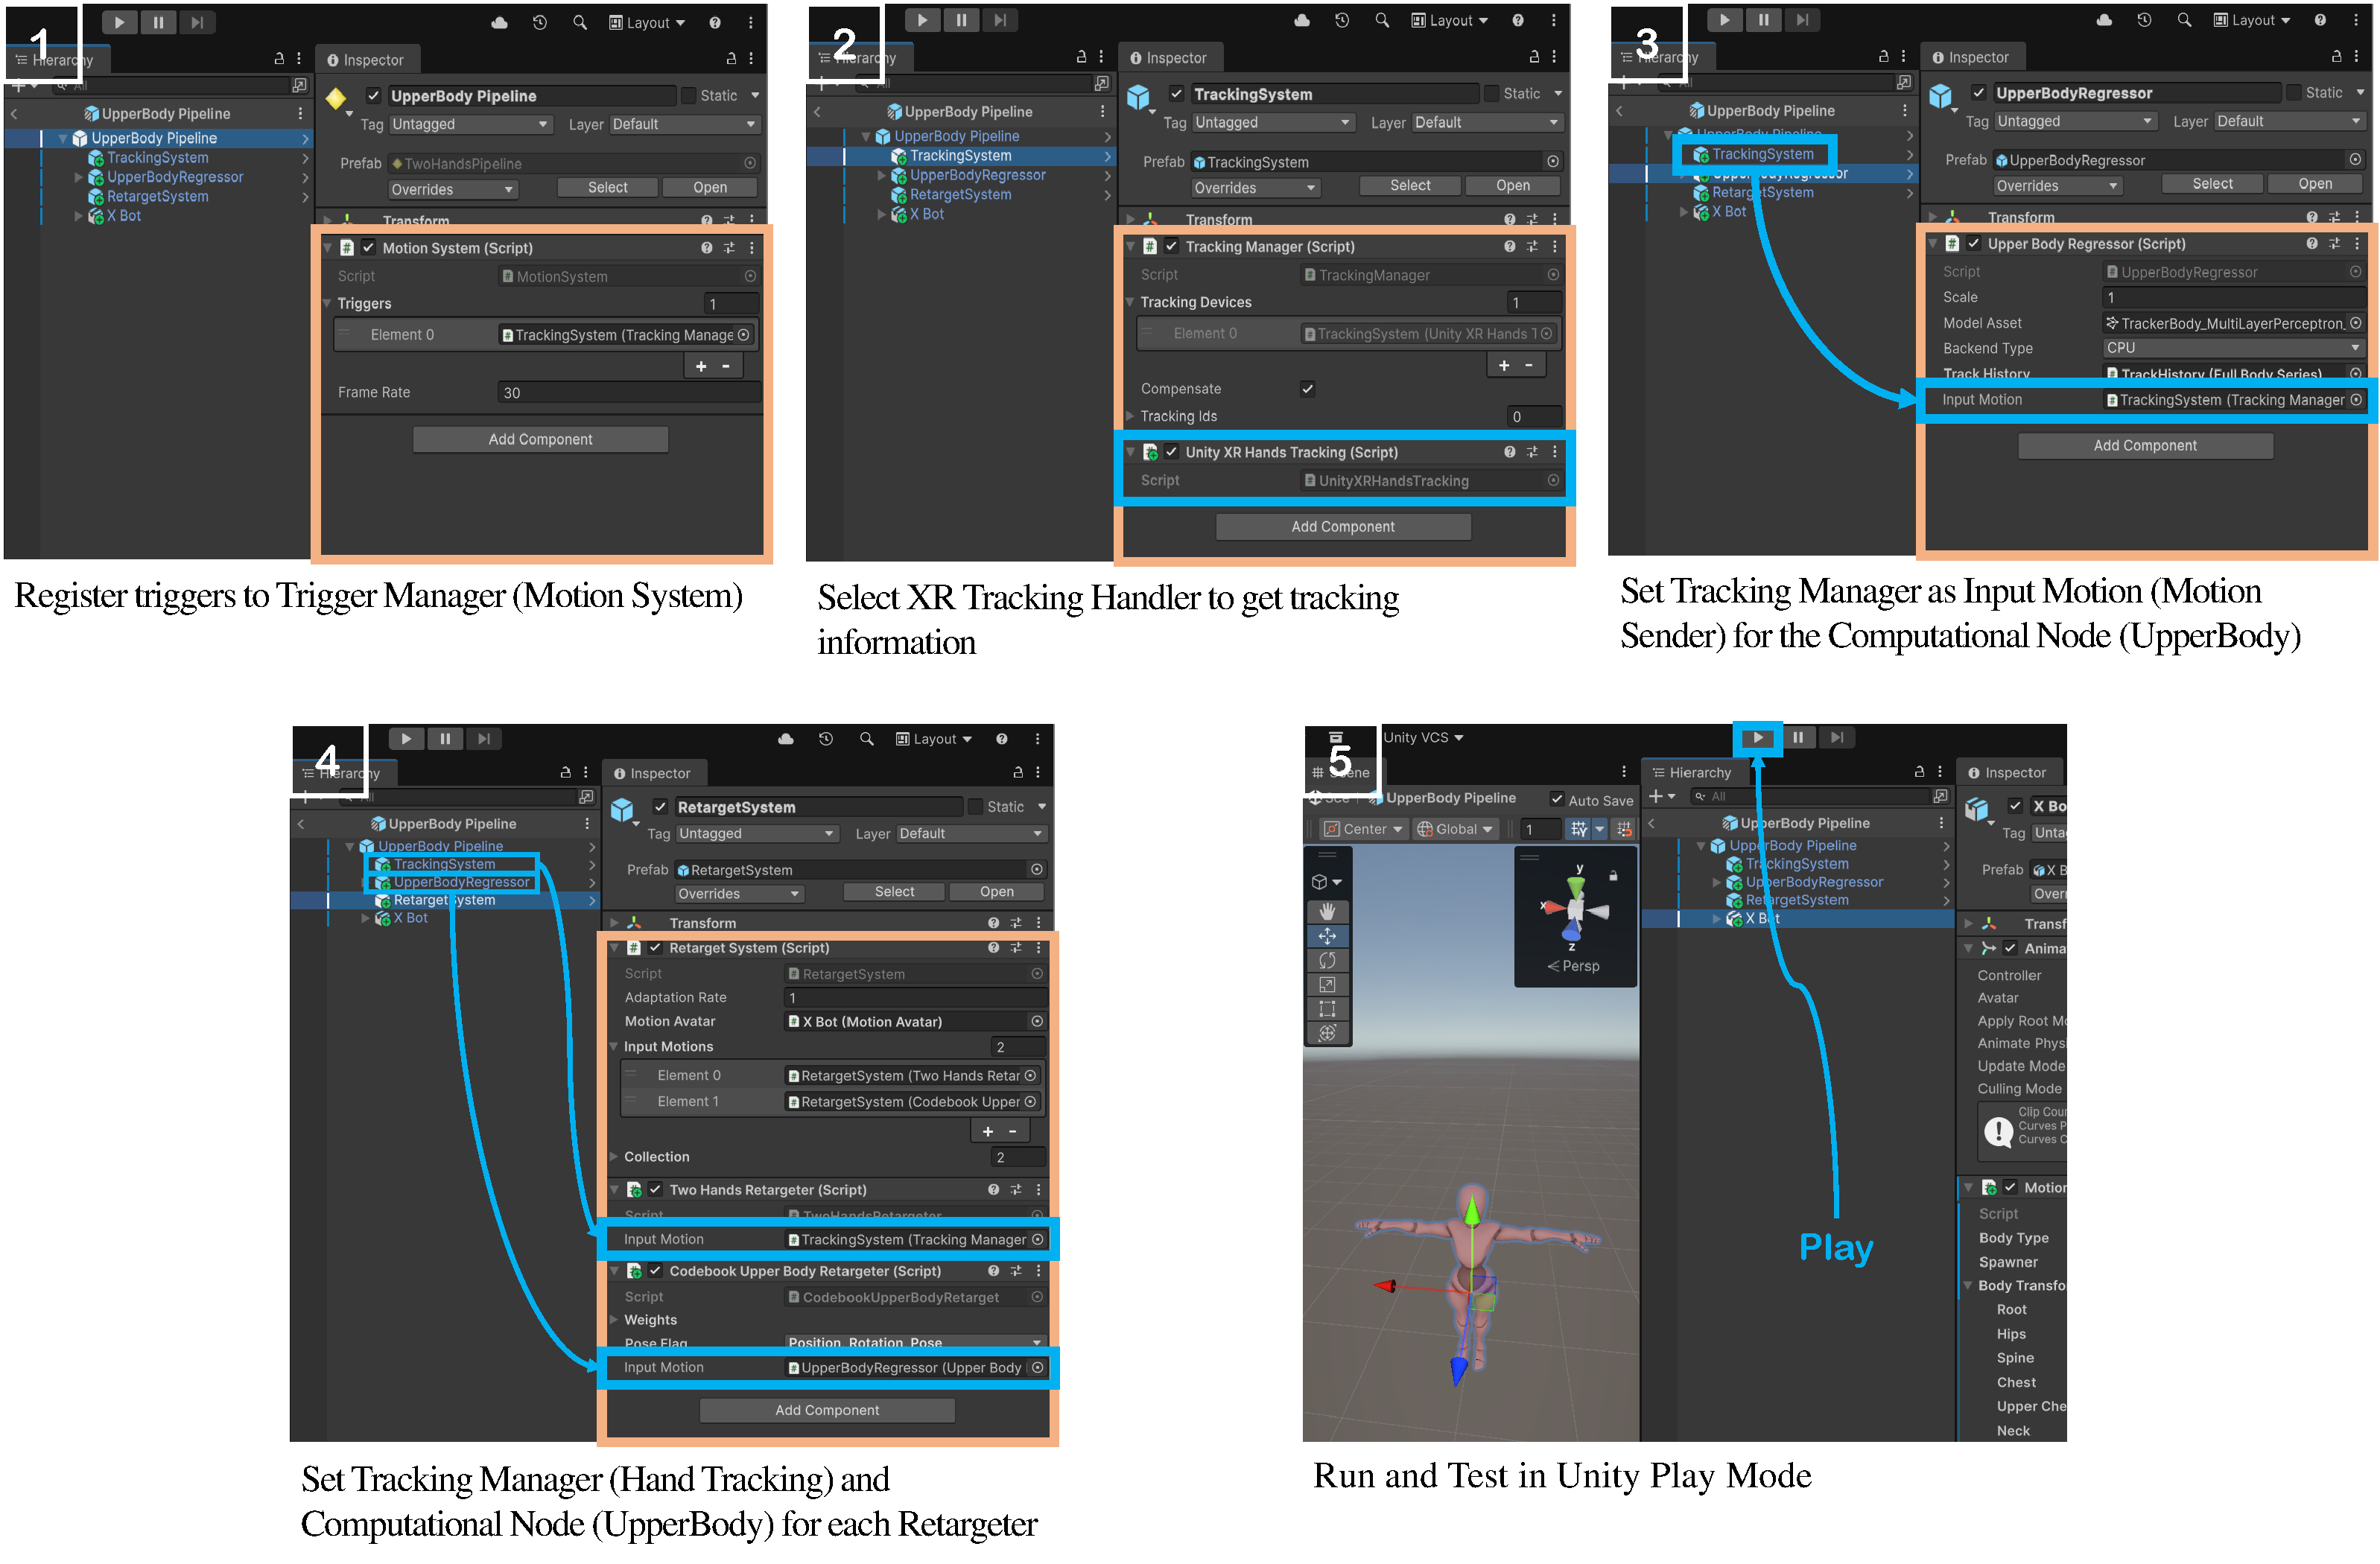
\includegraphics[width=0.95\textwidth]{figures/fig4-authoring.pdf}
  \caption{Unity workflow for two-hand \& upper-body configuring a MotionDAG pipeline.}
  \label{fig:authoring}
\end{figure*}


Unlike body skeleton retargeting, XR hand tracking presents unique challenges due to the lack of consistent reference frames across SDKs.
To address this, we employ a shape-correspondence principle that defines hand coordinate axes based on anatomical structure.
We construct a reference rotation frame for the wrist and each finger joint using outgoing directions from finger bones and lateral directions defined by neighboring fingers.
Let $\mathbf{R}_i = [\hat{\mathbf{x}}_i,\hat{\mathbf{y}}_i,\hat{\mathbf{z}}_i]$ denote the rotation reference frame for joint $i$,
then the axis of the frame can be determined by the origin, forward and lateral neighbor positions for segment $i$, respectively $\mathbf{p}_{i}^{(o)}$, $\mathbf{p}_{i}^{(f)}$, and $\mathbf{p}_{i}^{(l)}$ as follows.
\begin{align}
    \hat{\mathbf{x}}_i &= \frac{\mathbf{p}_{i}^{(l)}-\mathbf{p}_{i}^{(f)}}{\lVert \mathbf{p}_{i}^{(l)}-\mathbf{p}_{i}^{(f)}\rVert}, \\    
    \hat{\mathbf{z}}_i &= \frac{\mathbf{p}_{i}^{(f)}-\mathbf{p}_{i}^{(o)}}{\lVert \mathbf{p}_{i}^{(f)}-\mathbf{p}_{i}^{(o)}\rVert}, \\
    \hat{\mathbf{y}}_i &= s\;\frac{\hat{\mathbf{z}}_i \times \hat{\mathbf{x}}_i}{\lVert \hat{\mathbf{z}}_i \times \hat{\mathbf{x}}_i\rVert},
\end{align}
with $s=+1$ for left hands and $s=-1$ for right hands.
For the wrist joint $w$, denote its position as $\mathbf{p}_{w}^{(o)}$, the middle-finger proximal joint as
$\mathbf{p}_{w}^{(f)}$, and the index proximal joint as $\mathbf{p}_{w}^{(l)}$.
For each tracked segment $i$ (e.g., each phalanx along a finger chain), we define role-labeled points $\{\mathbf{p}_{i}^{(o)},\mathbf{p}_{i}^{(f)},\mathbf{p}_{i}^{(l)}\}$, where $(o)$, $(f)$, and $(l)$ denote the segment origin, its child-joint reference (toward the fingertip), and a lateral-neighbor reference, respectively.
The resulting alignment factors $\mathbf{A}_{i}$ mirror the body retargeting bases and feed the final multiplication $\mathbf{T}_{i,\mathrm{track}}(t)\mathbf{A}_{i}\mathbf{T}_{i,\mathrm{tgt}}^0$, so both body and hand retargeting share the same relative-transform structure.
By establishing these consistent hand frames for both the source tracking data and the target avatar's hand rig, the Retargeter computes relative rotations from the canonical hand pose to the current tracked pose.
This approach eliminates the need for manual rig configuration and handles variations for finger bone orientation, providing robust retargeting across diverse avatar hand representations.

